\chapter{Our Project}

\section{The Final Application}
Planly is a collabortive project management application built as a single page web application. When users type in the URL for Planly, they are taken to the application's homepage shown in \ref{homepage} The homepage featured an image of our application. It is very minimalistic as users need to have an account in order to use the application.

\begin{figure}[ht]
\centering
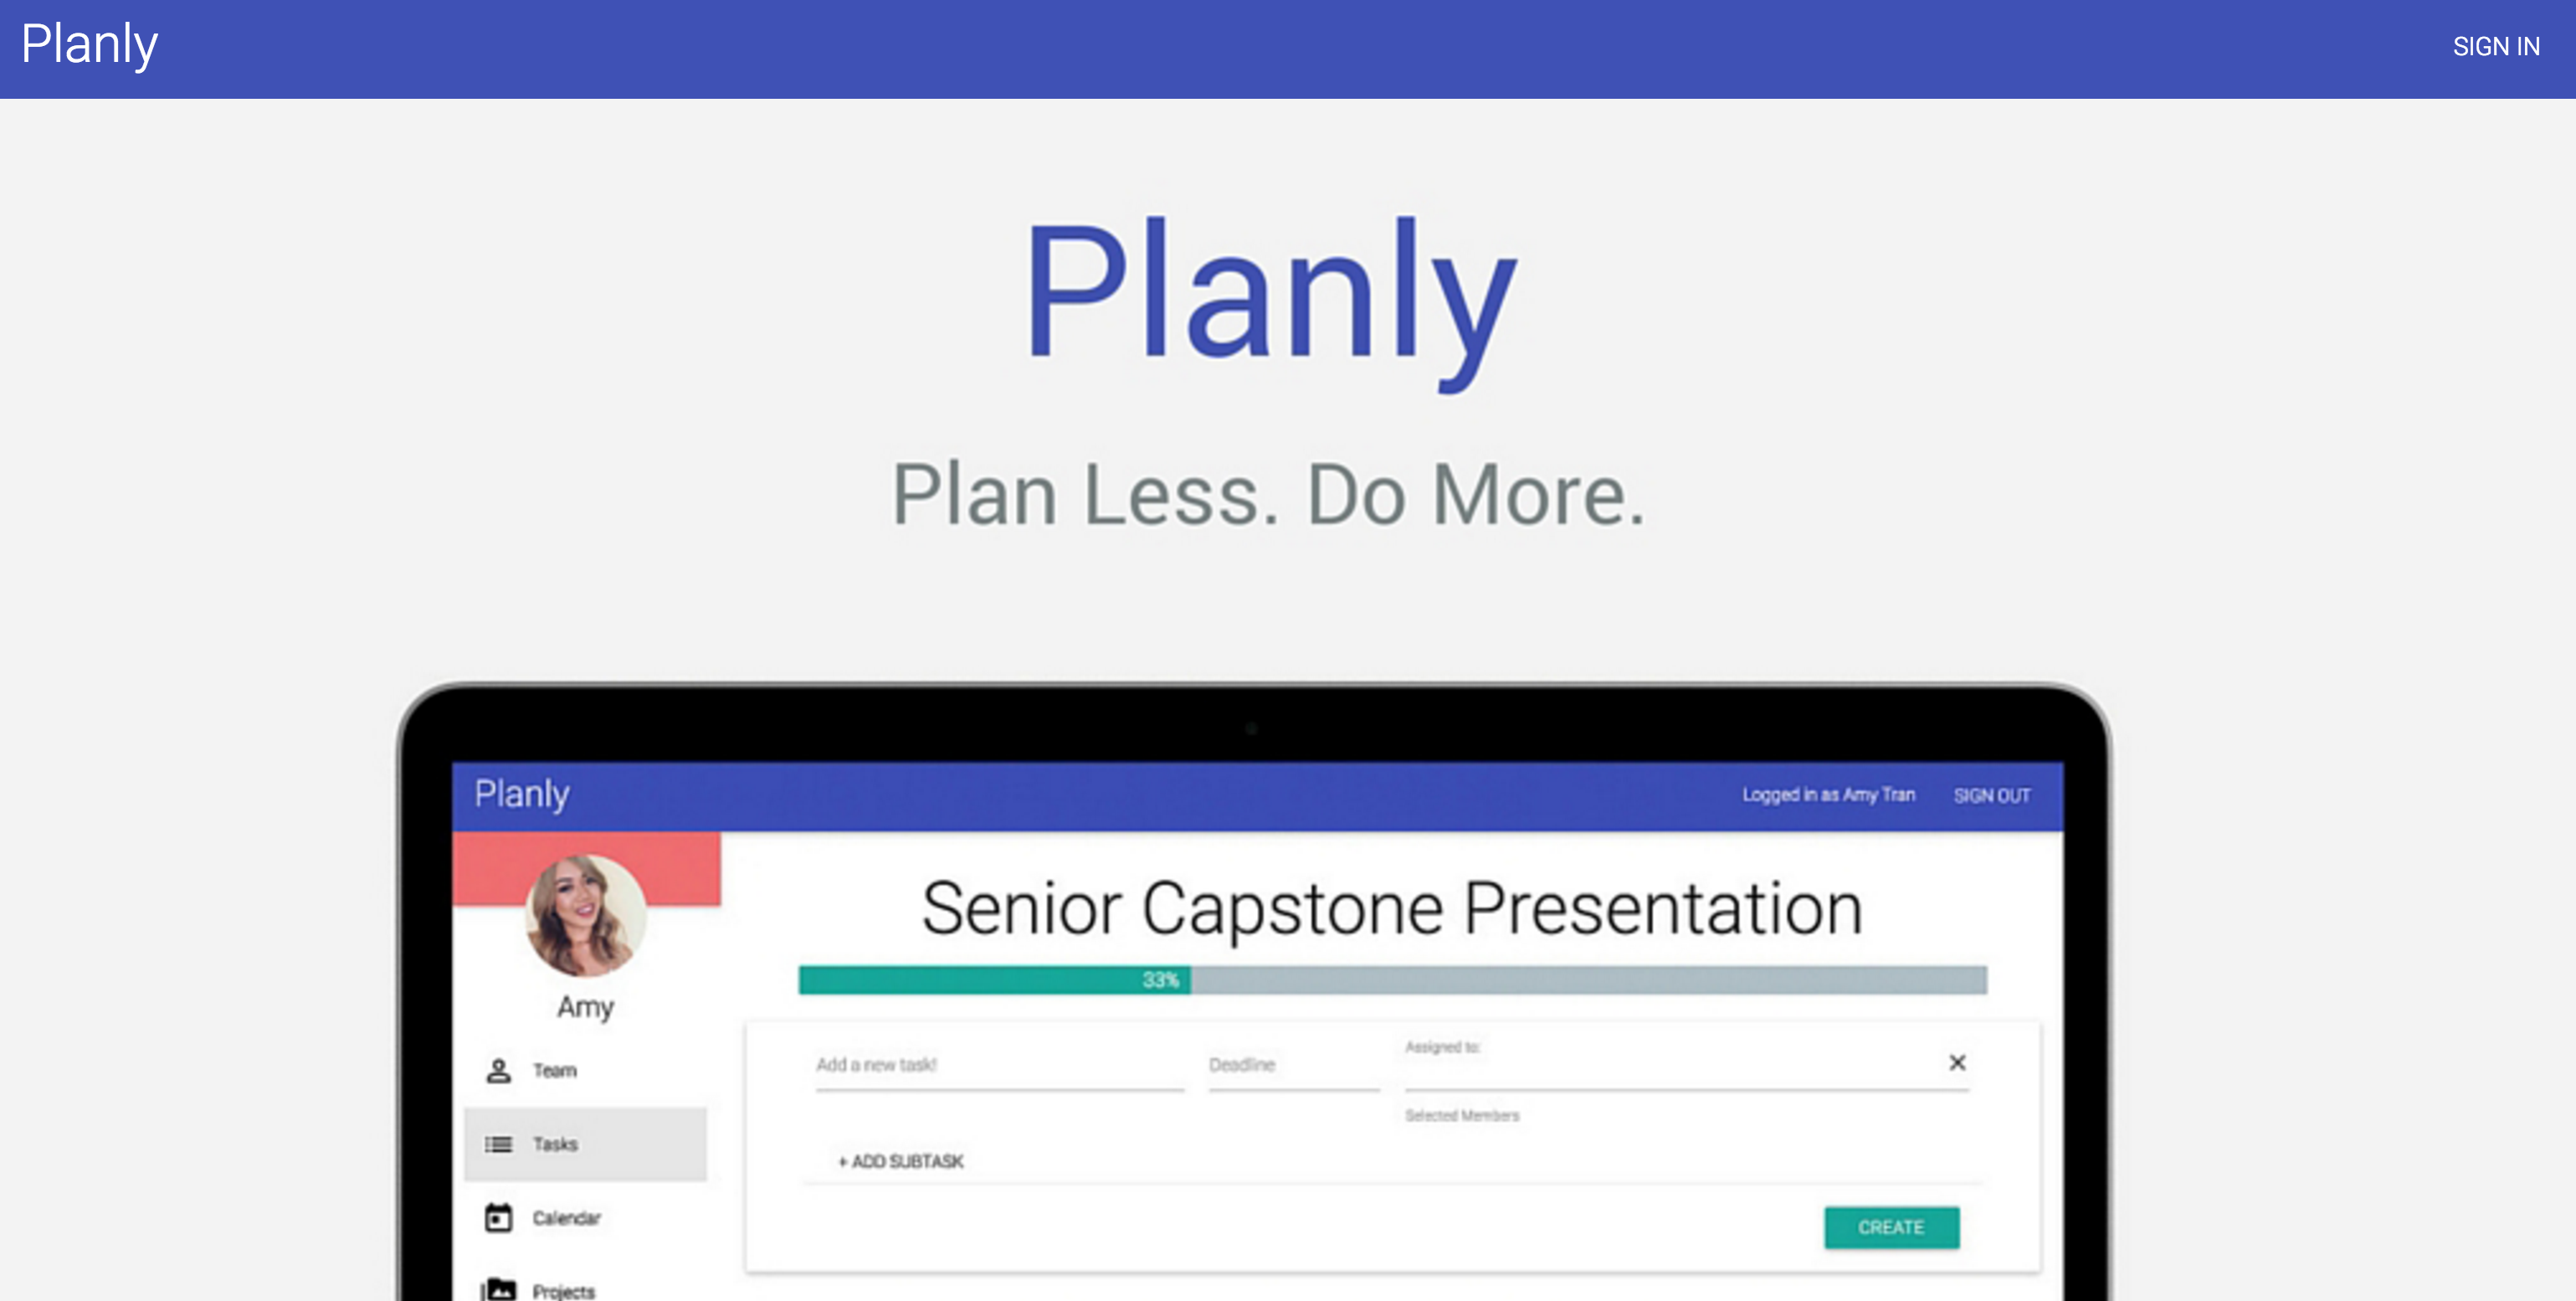
\includegraphics[width=\textwidth]{figure41.png}
\empuse{figure}
\caption{Homepage}
\label{homepage}
\end{figure}
\FloatBarrier

\subsection{Login}
In order to log in or sign up for Planly, users must select ``Sign In'' on the top right corner of the homepage. We provide users with three different methods to sign up for an account: Google, Facebook, or Email, shown in \ref{signin}. After a user has successfully logged in, he/she will be presented with the \emph{Projects} view. The \emph{Projects} view, seen in \ref{projectview}, hosts all of the user's projects as well as the members for each project. 

\begin{figure}[ht]
\centering
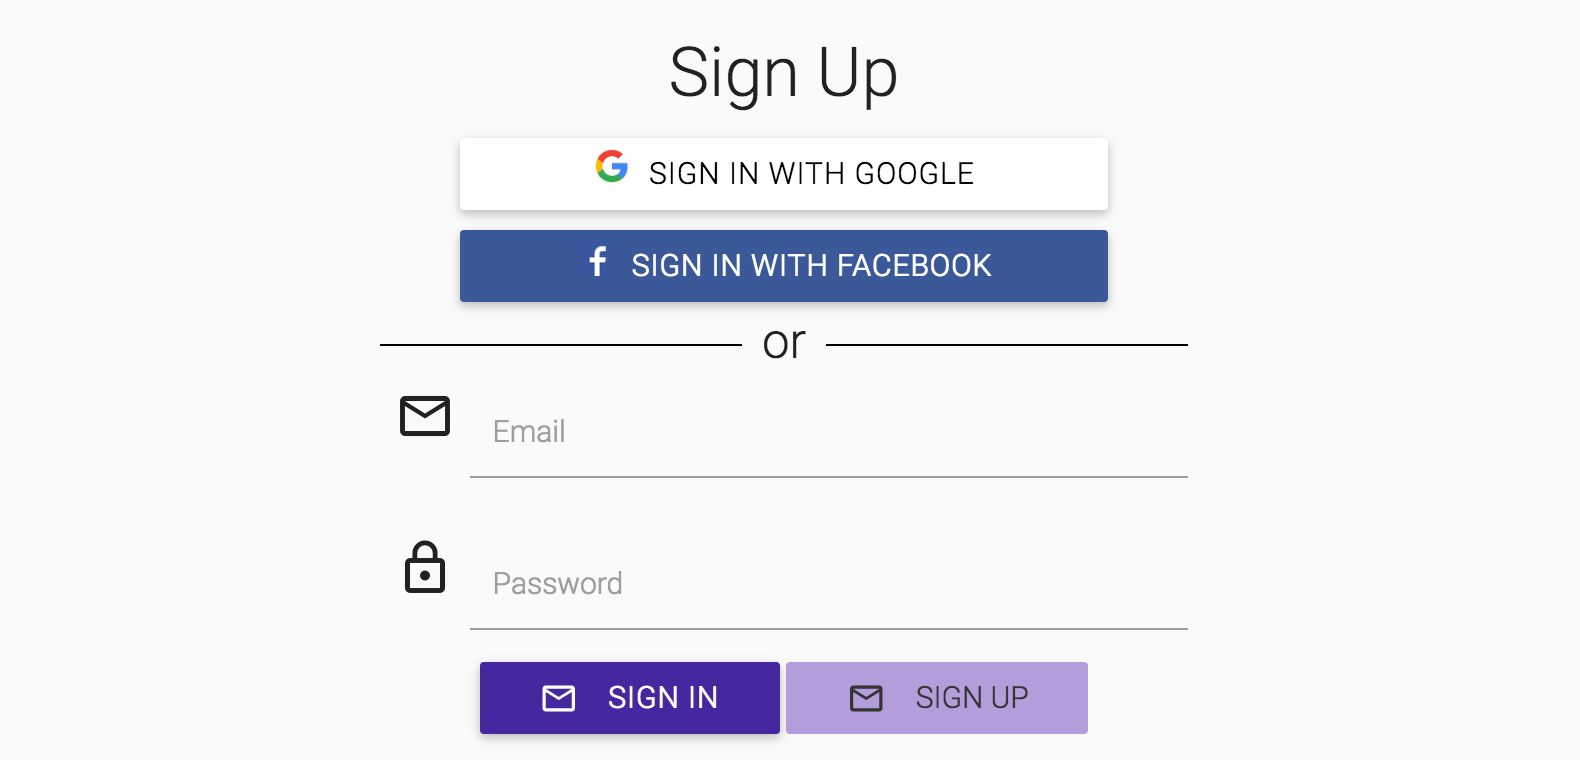
\includegraphics[width=\textwidth]{figure42.png}
\empuse{figure}
\caption{Sign In / Login Screen}
\label{signin}
\end{figure}
\FloatBarrier

\begin{figure}[ht]
\centering
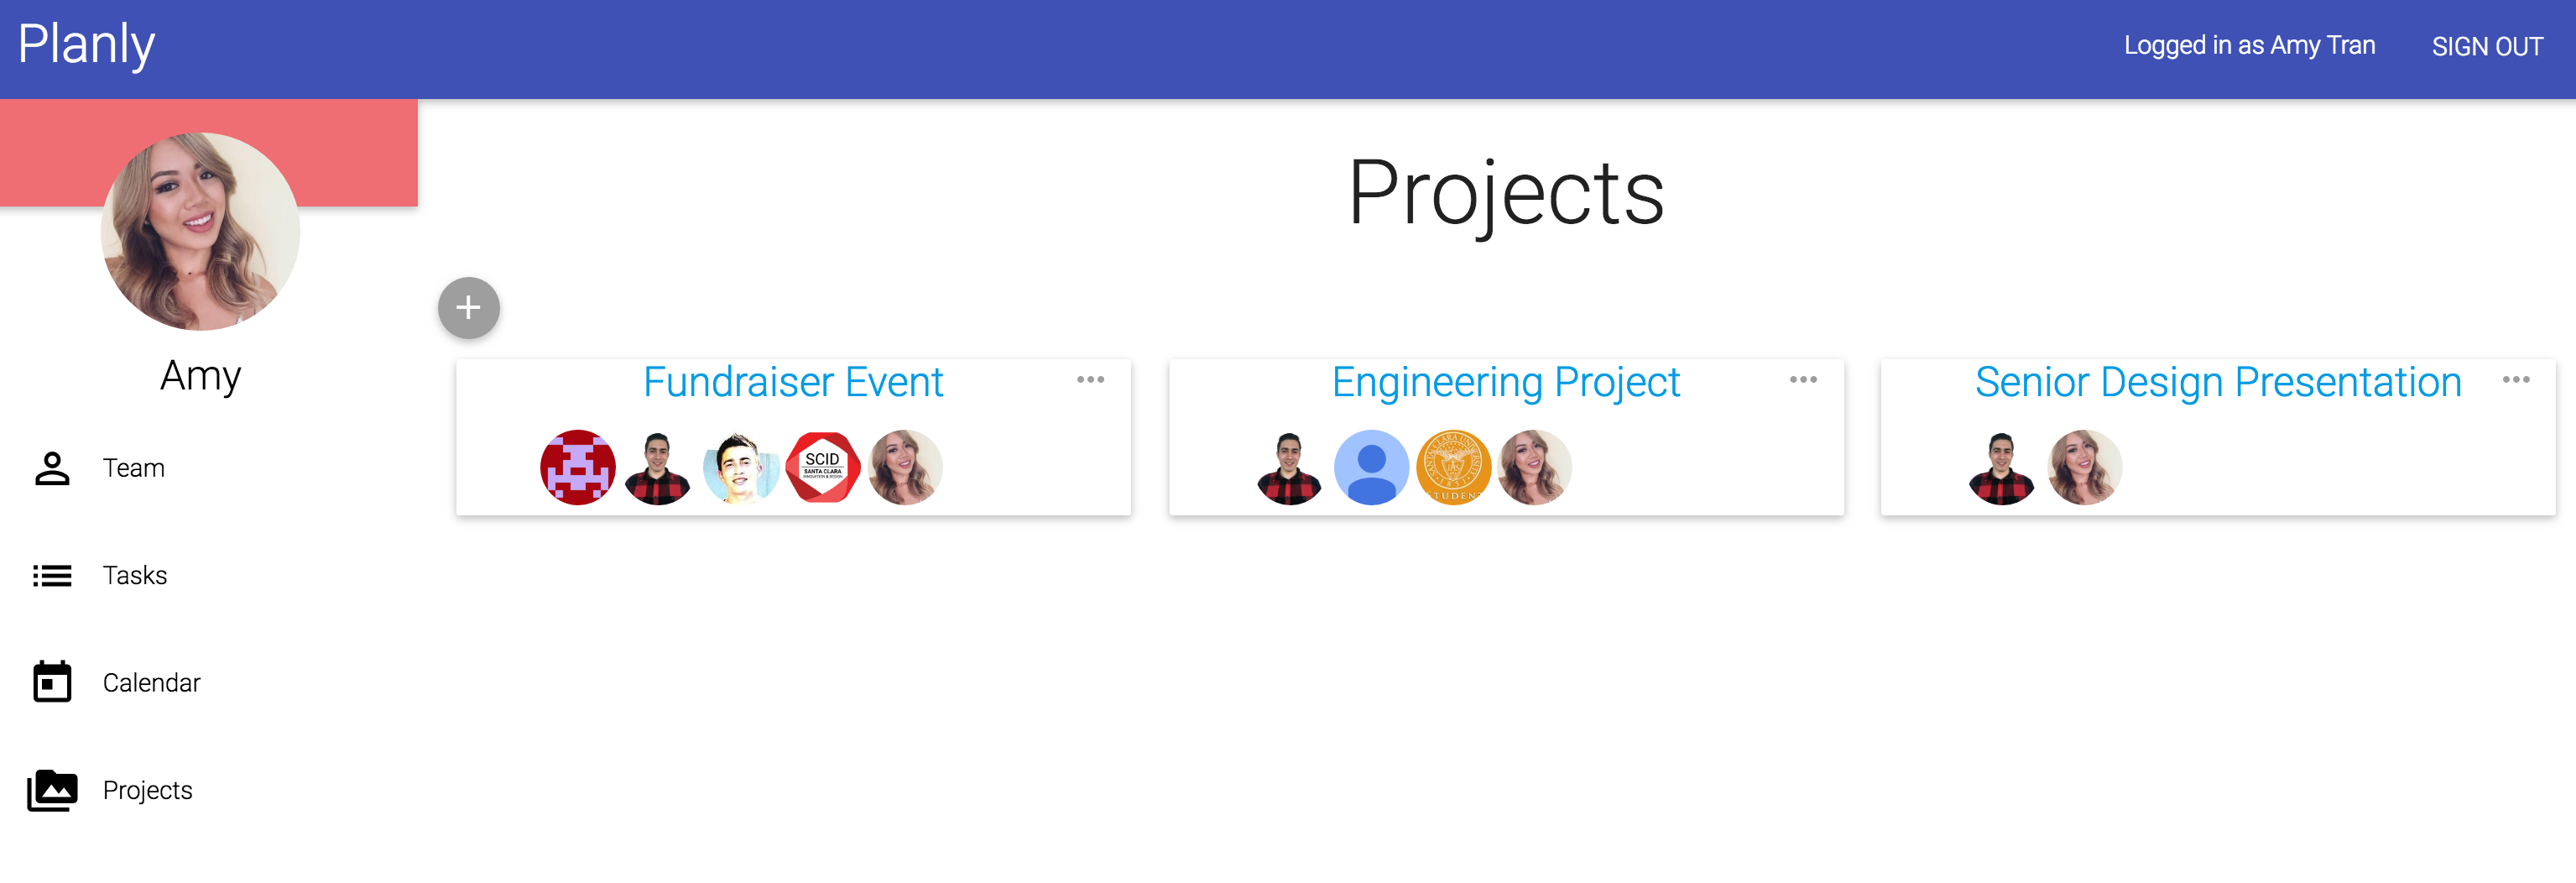
\includegraphics[width=\textwidth]{figure43.png}
\empuse{figure}
\caption{Projects View}
\label{projectview}
\end{figure}
\FloatBarrier

\subsection{Creating Projects and Teams}
From the \emph{Projects} view, users can create a new project as well as create teams for the project. By clicking on the + icon, users will activate the Project Creation form, depicted in \ref{projectcreationform}. The user needs to input the Project name, goal, deadline and team members. After completing the Project Creation form, users are given the option to create a team or to skip it at this time. 
\par If the user decides to create a team, he will need to enter the team name, description and team members.

\begin{figure}[ht]
\centering
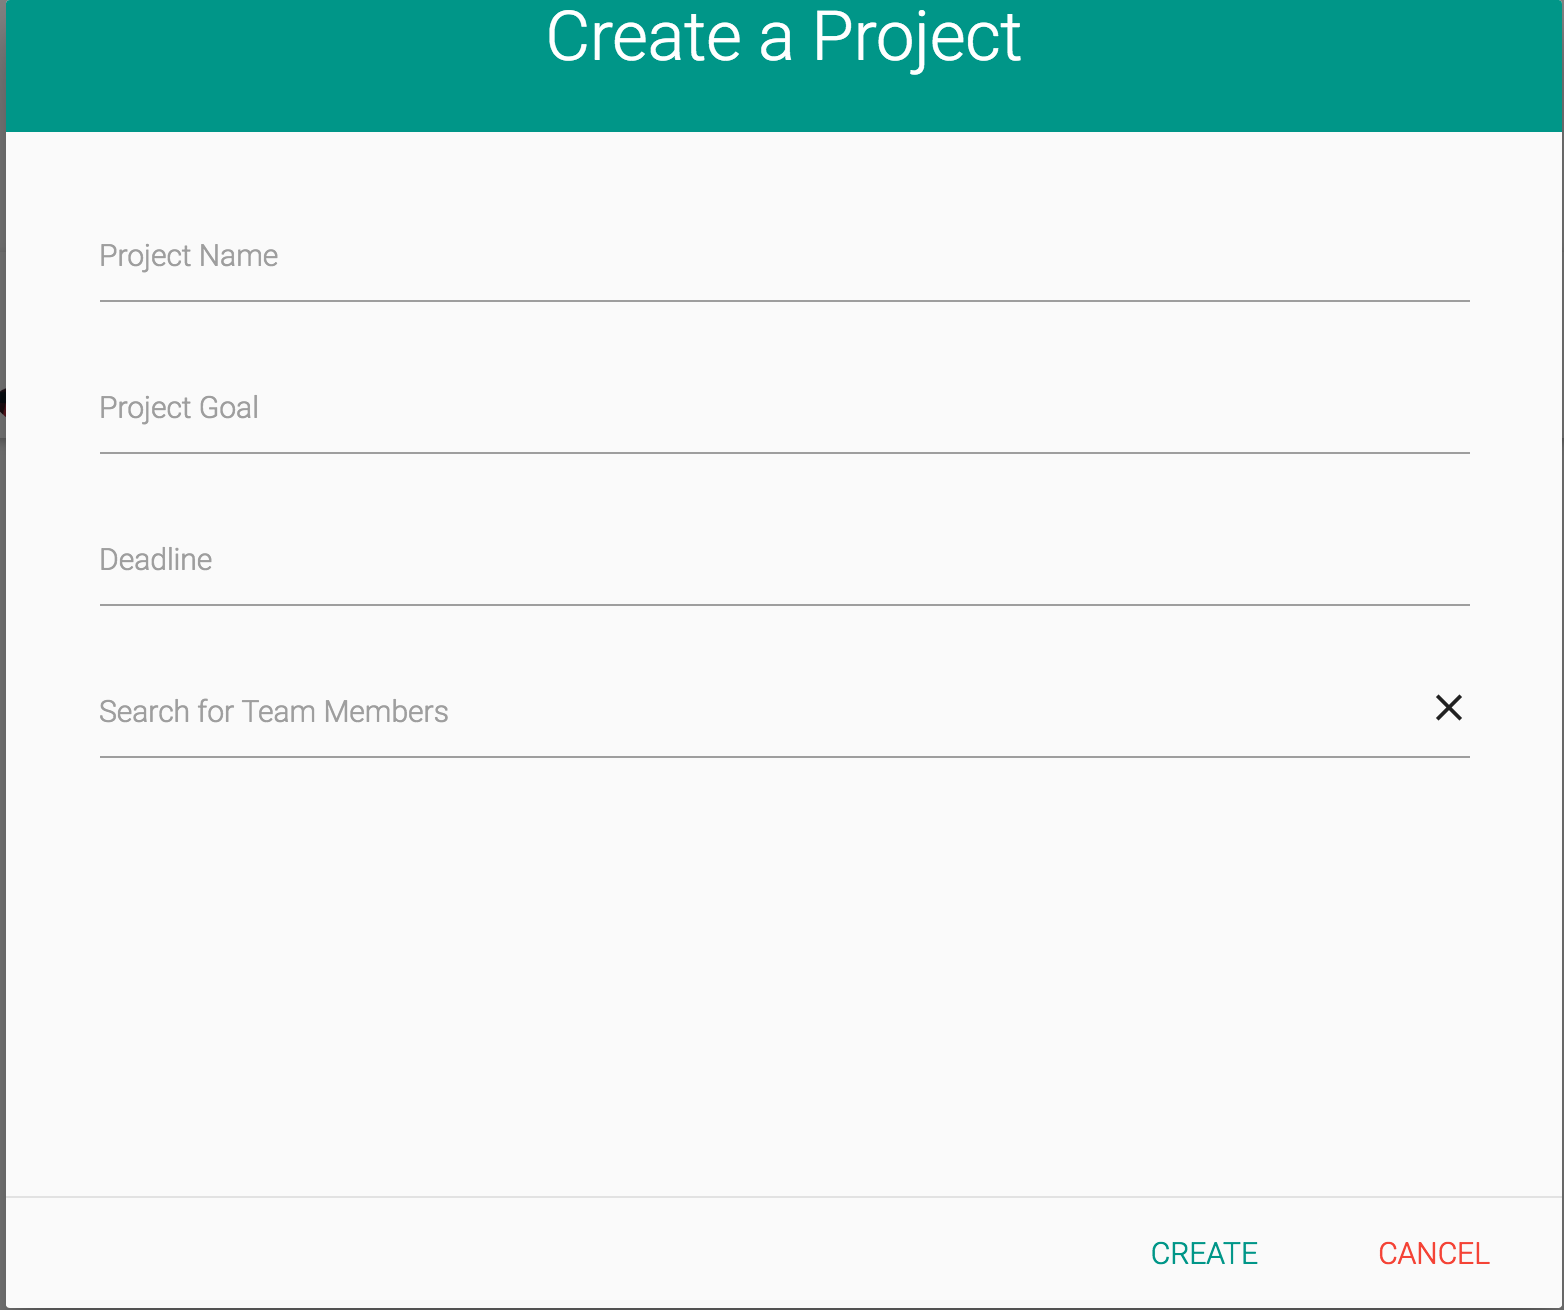
\includegraphics[width=\textwidth]{figure44.png}
\empuse{figure}
\caption{Project Creation Form}
\label{projectcreationform}
\end{figure}
\FloatBarrier

\subsection{Adding Tasks and Subtasks}
After the project has been created, users can now add task and subtask to the project. \ref{taskview} shows the \emph{Tasks} view. In the \emph{Tasks} view, users are presented with the project's name, progress bar, and a form to add tasks and subtasks. Once a user fills out the tasks form, he can then add a subtask or simply create the task. The task will appear on the screen with the task's deadline and who the task is assigned too. From there, users can click on the subtask icon to see the subtasks associated with the task or then can click the comment icon and post a comment. When a user marks a task as completed, the progress bar will change to reflect the progress of the project. 

\begin{figure}[ht]
\centering
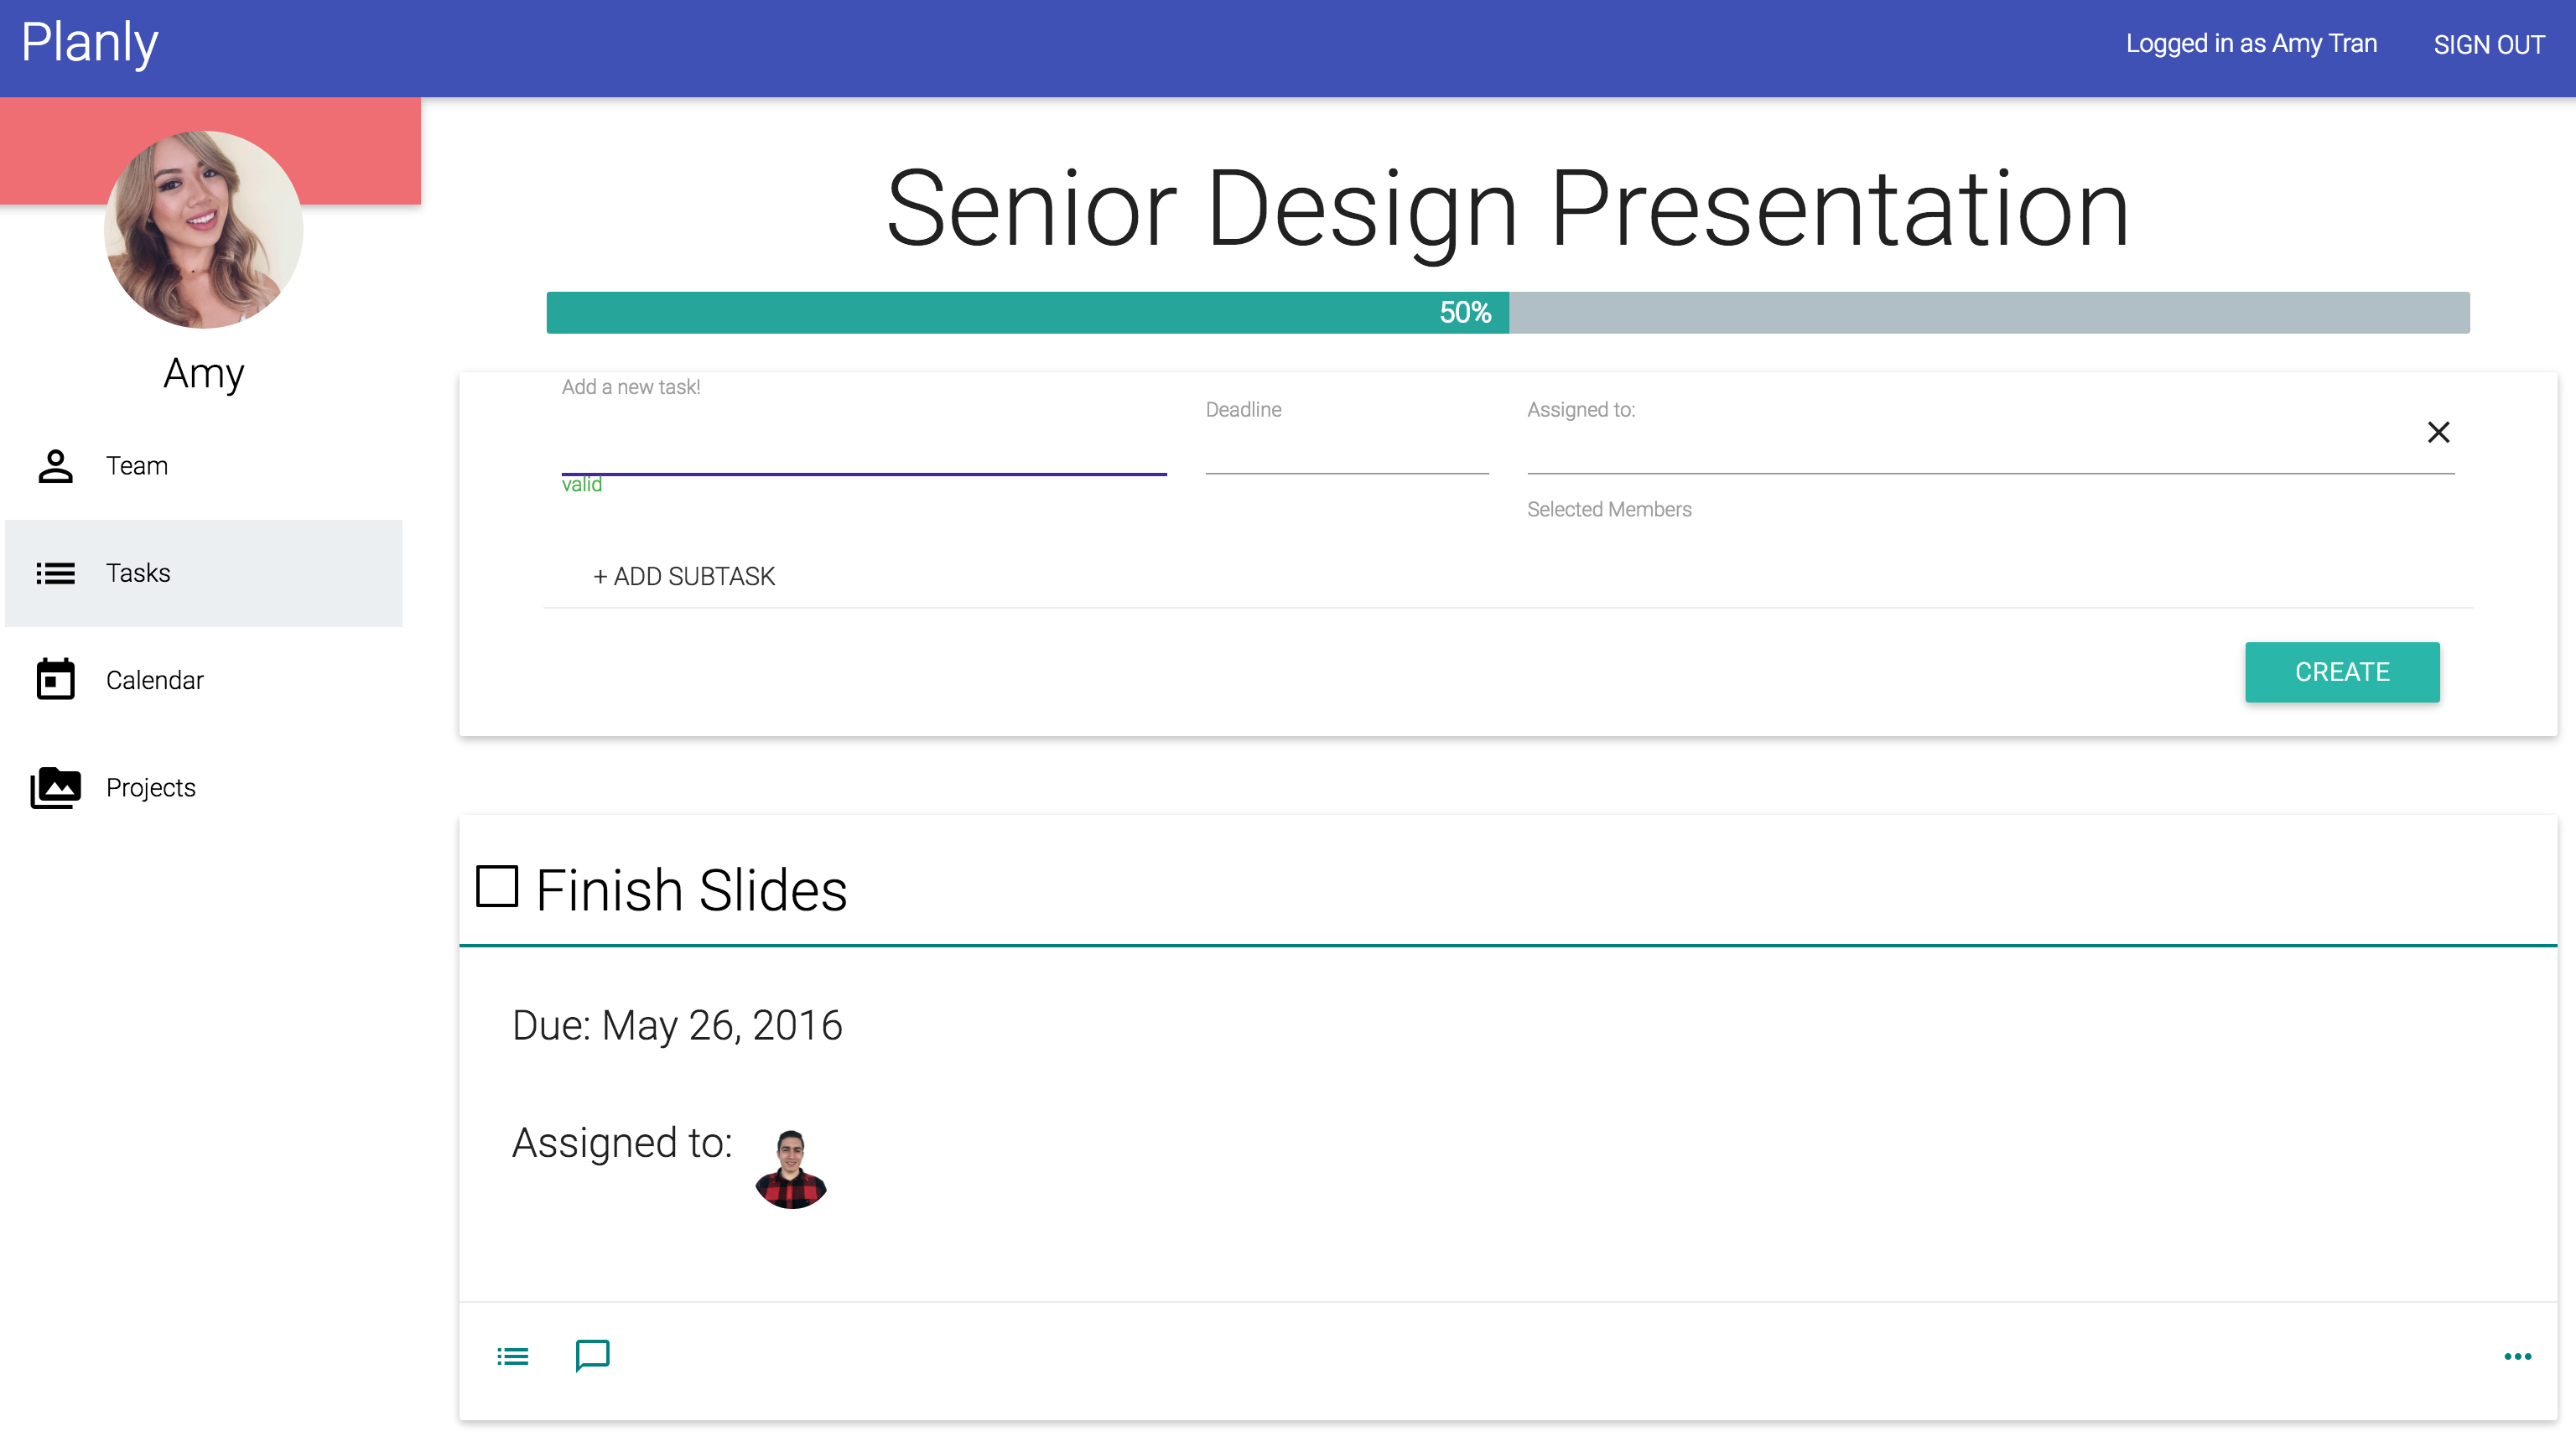
\includegraphics[width=\textwidth]{figure45.png}
\empuse{figure}
\caption{Task View}
\label{taskview}
\end{figure}
\FloatBarrier


\section{User Testing and Results}
After we completed Planly, we hosted a user testing session where we invited students to complete a series of tasks and provide us with their feedback. At the end of the test, we asked users to submit an anonymous survey. Figure 4.6 and Figure 4.7 shows our user testing results. 
\par Beginning with the system as a whole, from the user testing results, the majority of the users found Planly to be very usable system. To the question,``I found Planly to be a usable system", 55.5\% of users rated Planly as a 5, the highest score on our scale. As for the question `` I found Planly to be overly complex", a third of the users rated Planly a 1, meaning that they did not find Planly to be complex. However, a third of the users also answered with a score of 3, thus although most users found Planly to be usable, we acknowledge that there is still work to be done. 
\par Another question we asked in our survey was ``What are some areas of improvement for Planly" and users were allowed to select all features that applied. According to the results, we found that the features that needed the most improvement were task and subtasks. It is interesting observation is that tasks and subtasks were the last features we worked on prior to the testing, thus it makes sense that these features were the weakest.  
\section{Lessons Learned}
We want to highlight three important lessons that we learned while developing Planly: the importance of human centered design, the need for multiple system iteratations, and the neccesity to integrate early and often.

\subsection{Challenges}
\subsection{Future Work}

